\documentclass[11pt, a4paper]{article}
\usepackage[paper=a4paper, left=1.5cm, right=1.5cm, bottom=1.5cm, top=1.5cm]{geometry}
%
\usepackage[utf8]{inputenc}
\usepackage[spanish]{babel}
\newcommand\Frac[3][]{ #1 #2\color{black}\above 0.4pt \normalcolor #1#3}
\usepackage{amsmath,amssymb}
\usepackage{xcolor}
\usepackage{caratula/caratula}
\usepackage{bm}
\usepackage{float}
\usepackage{listings}
\usepackage{color}
 
\definecolor{codegreen}{rgb}{0,0.6,0}
\definecolor{codegray}{rgb}{0.5,0.5,0.5}
\definecolor{codepurple}{rgb}{0.58,0,0.82}
\definecolor{backcolour}{rgb}{0.95,0.95,0.92}
 
\lstdefinestyle{coding}{
    backgroundcolor=\color{backcolour},   
    commentstyle=\color{codegreen},
    keywordstyle=\color{magenta},
    numberstyle=\tiny\color{codegray},
    stringstyle=\color{codepurple},
    basicstyle=\footnotesize,
    breakatwhitespace=false,         
    breaklines=true,                 
    captionpos=b,                    
    keepspaces=true,                 
    numbers=left,                    
    numbersep=5pt,                  
    showspaces=false,                
    showstringspaces=false,
    showtabs=false,                  
    tabsize=1
}
 
\lstset{literate=%
{$}{{\$}}1
{å}{{\aa}}1
{ø}{{\o}}1
{Æ}{{\AE}}1
{Å}{{\AA}}1
{Ø}{{\O}}1
}
\lstset{extendedchars=\true}
\lstset{inputencoding=ansinew}
 
 
\lstset{style=coding}

\begin{document}

\titulo{Trabajo Práctico 2 }
\fecha{Domingo 15 de Abril de 2018}
\materia{Organización del Computador II}

\integrante{Agustín Sansone}{99/17}{agustinsansone7@gmail.com}
\integrante{Kennedy Rios Cuba}{503/15}{wrios@dc.uba.ar}
\integrante{Paulo Ballan}{381/15}{ballanpaulo25@gmail.com}

%Carátula
\maketitle
\newpage

%Indice
\tableofcontents
\newpage

%Introduccion
\section{Introducción}
Este trabajo consiste en implementar filtros gráficos utilizando el modelo de procesamiento SIMD. De esta manera procesaremos, por ejemplo, 4 píxeles de una imagen al mismo tiempo. Se busca encontrar una mejora significativa entre la utilización de dichos registros $XMM$ contra el proceso provisto en el lenguaje de programación $C$. 

% Esta parte no me cierra, la puedo mejorar.
Se abarcaran 4 conocidos filtros de imágenes distintos provistos por la cátedra. Estos filtros son:

\subsection{Tres Colores}

Este filtro realiza un cambio en los colores de cada pixel en base a 3 colores fijos que son: 

\begin{itemize}
  \item Crema (R: 236, G: 233, B: 214)
  \item Verde (R: 0, G: 112, B: 110)
  \item Rojo (R: 244, G: 88, B: 65)
\end{itemize}

La definición de cual de estos colores se va a elegir depende directamente del brillo que se calcula con la siguiente fórmula:

$W = \floor{\frac{(Pixel_r + Pixel_g + Pixel_b)}{3}}$

Para cada píxel conseguiremos $W$ que luego definirá cual de los 3 colores mencionados anteriormente es el correcto para utilizar.
Estos colores representan una $3/4$ del nuevo color que se va a obtener para cada píxel.

\subsection{Efecto Bayer}
\subsection{Cambia Color}
\subsection{Edge Sobel}

%Agregar imágenes lindas para cada filtro, quizás algunas de internet o algunas que le hagamos posta el filtro.
El filtro Tres Colores es usado para ...\\
El filtro Bayer es usado para ... . La razón de que se use mayor cantidad de puntos verdes es que el ojo humano es más sencible a ese color.\\
EL filtro Cambia Colores es usado para ...\\
El cuarto filtro es Edge Sobel, el cual utiliza la vecindad de Moore para hacer una aproximaci\'on de las derivadas parciles, este filtro es \'util para poder detectar los bordes de la imagen.\\


\newpage

%Fuerza Fruta
\section{Desarrollo}
\vspace{5px}
\subsection{Tres Colores} 

Dentro de este filtro elegimos tomar de a 4 píxeles donde dividimos en 2 partes el cálculo de estos mismos. 
La primera parte consiste en calcular $W$, para cada uno de los píxeles. Para esto duplicamos los bytes de colores individuales en 4 registros distintos para luego sumarlos y obtengamos algo como:

\begin{table}[h]
\begin{center}
\begin{tabular}{|c|c|c|c|c|}
\hline
      & dword     & dword     & dword     & dword     \\ \hline
xmm1: & R     & R     & R     & R     \\ \hline
+     & +     & +     & +     & +     \\ \hline
xmm2: & G     & G     & G     & G     \\ \hline
+     & +     & +     & +     & +     \\ \hline
xmm3: & B     & B     & B     & B     \\ \hline
=     & =     & =     & =     & =     \\ \hline
xmm1: & R+G+B & R+G+B & R+G+B & R+G+B \\ \hline
\end{tabular}
\end{center}
\end{table}

De esta manera obtenemos el cálculo $R+G+B$ de 4 píxeles. Una vez obtenida la suma anterior, necesitamos dividirla por 3 para obtener el $W$ deseado. Para evitar la pérdida de precisión en este pasó, convertimos estos valores a $single$ $precision$ $floats$. Una vez realizada esta conversión y la división volvemos a formatear a $int$:

\begin{table}[h]
\begin{center}
\begin{tabular}{|c|c|c|c|c|}
\hline
      & dword     & dword     & dword     & dword     \\ \hline
xmm1: & W     & W     & W     & W     \\ \hline
\end{tabular}
\end{center}
\end{table}

Para elegir entre los colores: $crema, rojo, verde$ en cada pixel se realiza una serie de comparaciones para evaluar el valor correcto. Para calcular estos valores se pasa por comparaciones de los 3 colores predefinidos ($crema$, $rojo$ y $verdes$). Estos mismos valores se encuentran cargados en la sección de .data ya multiplicados por 3, ya que el valor solo se utiliza así. Por lo tanto para ahorrar instrucciones se carga en memoria de antemano. 

Se decidió realizar primero las sumas de cada píxel antes de realizar la división por 4 para evitar perder precisión. Esto mismo nos genera el problema de posibles overflow en el único byte con el que veníamos trabajando, ya que cada byte de los colores predefinidos es multiplicado por 3 y eso de por si puede generar overflow. Por lo que se decidió realizar los siguientes pasos para el procesamiento de cada color:

\begin{itemize}
  \item Dividimos el proceso de los 4 píxeles en dos, en pos de evitar overflow por lo primero tomaremos los dos primeros píxeles extendidos. Realizamos esta división de procesamiento para evitar overflow, ya que al multiplicar por 3 las constantes que tenemos predefinidas algunas superan los 2 bytes disponibles que tenemos, y si en adición sumamos W esto solo empeora la situación. Cabe aclarar que la división por 4 para cada píxel la realizamos luego de sumar ambos términos para no perder precisión.
  
  \item Miremos especialmente una iteracion para uno de los colores predefinidos: A los dos píxeles primero agregamos los correspondientes valores de $W$, los dividimos por 4 y al finalizar realizamos als comparaciones para elegir cuales de estos colores deberían llegar el color predefinido actual. Realizamos el mismo procedimiento para los segundos píxeles. 
  Este mismo proceso se realiza una vez para cada uno de los colores predefinidos $crema$, $rojo$ y $verdes$.
\end{itemize}

Una vez realizado este procesamiento obtenemos el siguiente registro:


\begin{table}[h]
\begin{center}
\begin{tabular}{|c|c|c|c|c|}
\hline
      & dword     & dword     & dword     & dword     \\ \hline
xmm1: & (CVR + W)/4     & (CVR + W)/4     & (CVR + W)/4     & (CVR + W)/4     \\ \hline
\end{tabular}
\end{center}
\end{table}

Siendo CVR el color correspondiente para cada pixel.
Una vez obtenido este resultado escribimos en memoria el dato, para luego continuar ciclando la imagen. 


\subsection{Efecto Bayer}

Sobre este filtro dividimos las iteraciones en 2 partes una para cada fila:

\begin{itemize}
  \item En la primera tomaremos el patrón $Azul$ y $Verde$
  \item Y en la segunda tendremos el patrón $Verde$ y $Rojo$
\end{itemize}

Cabe destacar que tomamos en orden inverso los patrones a diferencia de los que se muestran en la imagen de ejemplo ya que se comienza desde el borde inferior derecho.

En el ciclo principal del filtro tomamos de a 2 filas:


\begin{table}[h]
\begin{center}
\begin{tabular}{|c|c|c|c|c|}
\hline
 Rojo   & Verde &  Rojo   & Verde & ...    \\ \hline
 Verde  & Azul & Verde  & Azul & ...   \\ \hline
\end{tabular}
\end{center}
\end{table}

Dentro de estos mismos, aplicamos un ciclo específico para cada una de las filas. Tomando por ejemplo la primera:

\vspace{6px}
\begin{center}
\includegraphics[width=10.5cm, height=1.5
cm]{images/efectobayer_unafila.png}
\end{center}
\vspace{6px}

Cuando tomamos esta fila comenzaremos a iterar de a 4 píxeles uno trabajando simultáneamente para ir filtrando los colores de estos píxeles utilizando la instrucción $shuffle$ para eliminar los demás colores. De esta manera completamos toda la fila.
Una vez completada esta fila se procede de manera similar con la siguiente fila 


\subsection{Cambia Color}

Para comenzar este filtro primero calculamos los valores de $N_r$, $N_b$, $N_b$, $C_r$, $C_g$, $C_b$, $lim$ a partir de los parámetros estableciendo registros $XMM$ llenos de estos mismos valores para así poder trabajar de a 4 píxeles a la vez. 

Una vez guardados los valores mencionados comenzaremos a ciclar sobre la imagen trayendo de a 4 píxeles. Paso siguiente, se calculo paso a paso el valor de $d$ para cada uno de estos píxeles con los siguientes pasos:

%Acá voy a agregar alguna manera bonita de poner los xmm, la estoy pensando todavía
\begin{itemize}
  \item Calcular los $\Delta B$, $\Delta R$, $\Delta G$ para cada píxel, por lo que obtendremos algo similar a $xmm = | \Delta R | \Delta R | \Delta R | \Delta R |$ para cada color. Este proceso se realiza en $int$ hasta la unión de todas las sumas que contienen ya que nunca superamos 1 byte en cada $dword$ que manejamos. Antes de realizar los últimos pasos para calcular $d$ y $c$, convertimos a float para no perder precision en la división por 256 que se encuentra adento, y tampoco para saturar ya que la suma de todos los valores antes de aplicar la raíz cuadrada podría saturar. Cabe destacar que también se pasa a float para calcular correctamente la raíz cuadrada. 
  \item El siguiente paso es calcular el valor designado en caso de que $d<lim$. Este mismo se calcula con 4 píxeles también y para cada uno realizamos las operaciones para generar $1-c$ y $N_r,N_b,N_g$ de cada byte del píxel, antes de multiplicar $1-c$ por cada respectivo valor, pasamos a float para no perder precisión. 
\end{itemize}

Una vez terminados estos pasos tenemos el resultado procesado de 4 píxeles que volvemos a dejar en memoria.


\subsection{Edge Sobel}
El algoritmo comenzara llenando la parte que se procesa (toda la matriz, excepto los bordes),
y luego completara los bordes de la matriz con 0.
Tiene cuatro diferentes tipos de iteraciones y un caso que es tratado de forma diferente.
\begin{itemize}
\item Llenado de la matriz con los pixeles procesados, se excluyen los bordes pues no se pueden aplicar los operadores.
\item Llenado de la última fila a procesar.
\item Llenado de los bordes de los costados.
\item El ultimo caso es para poder llenar la primer fila y la ultima con ceros, la forma de iterar es la misma pero cambia el lugar desde donde inicia cada una.
\end{itemize}
\subsubsection{Llenado de los pixeles procesados usando parte baja de un xmm} Se tomara la parte baja de un registro xmm y los 8 bytes de la parte baja serán extendidos a 8 words para que al hacer las cuentas no perdamos precisión, como se calcularán 4 pixeles, estaremos trabajando con 6 bytes, los 10 bytes restantes no se utilizarán. Esto solo sirve para llenar parte de la matriz, por que al querer seguir iterando, llegaremos a la última posición y necesitariamos leer 10 bytes demás, pero nos saldriamos de la matriz.

\subsubsection{Llenado de los pixeles procesadosusando parte alta de un xmm} Responde al problema que surgio anteriormente, entonces ahora al leer en un registro xmm tranjaremos con la parte alta, como necesitamos procesar 4 pixeles a la hora de acceder a la matriz necesitaremos estar 10 bytes (posiciones) atras, asi poder acceder a los 6 bytes con los que se procesan 4, luego por la forma en como iniciamos y dado que la cantidad de pixeles en la fila es muliplo de 8, no podremos  procesar los dos ultimos bytes y estos se harán como caso aparte.




\subsubsection{Llenado de los bordes de los costados} La matriz es accedienda desde último byte de la primer fila, copia su valor en un xmm, hace un shift de 2 bytes para poner los 2 primeros bytes en 0 y luego un shift de 2 bytes para reacomodar, con esto se puso en 0 los 2 byte de los costados, luego se incementa en cantidad de columnas a la posición y se procede de la misma forma hasta llegar a la ante-ultima fila.

\subsubsection{Llenado de los bordes superior e inferior}
	Para la \textbf{primer fila}, primero se lee con el registro xmm y se shiftean 8 bytes, se divide la cantidad de columnas por 8 y se procede a iterar cantidad de (cantidad de pixeles en fila/8) -1 para poder llenas la primer fila.
	Para la \textbf{ultima fila}, se lee desde 8 bytes antes y se hace un shift para poder poner en 0 los primeros 8 bytes de la ultima fila, luego se procede a iterar cantidad de (cantidad de pixeles en fila/8) -1 para poder llenar la matriz.


%\newpage

%Backtracking
\section{Experimentación}
En la siguiente experimentación realizaremos comparaciones entre el código escrito en ASM contra el escrito en C++ con optimización nivel 3.

Para medir el rendimiento usaremos la cantidad de ciclos de ejecución, en particular se tomara la mediana de las mediciones.

Se útilizara el registro Time Stamp Counter (TSC) que es global del procesador y se ve afectado por una serie de factores, como por ejemplo el scheluder para realizar un cambio de contexto, esto implicará contar muchos más ciclos (outliers) que si nuestra función se ejecutara sin interrupciones, con lo cual se decidió tomar la mediana que es más robusta dadas las condiciones. En los experimentos contemplaremos el valor de un lado de la imagen, que interpretamos como matriz, en el eje X y en el eje Y tomaremos la mediana de la cantidad de clocks que toma dicha matriz con la función.



\subsection{Tres Colores}

El primer experimento comienza con la función de Tres Colores. Uno de las primeras aproximaciones de los resultados que estimamos fue una mejora

\vspace{6px}
\begin{center}
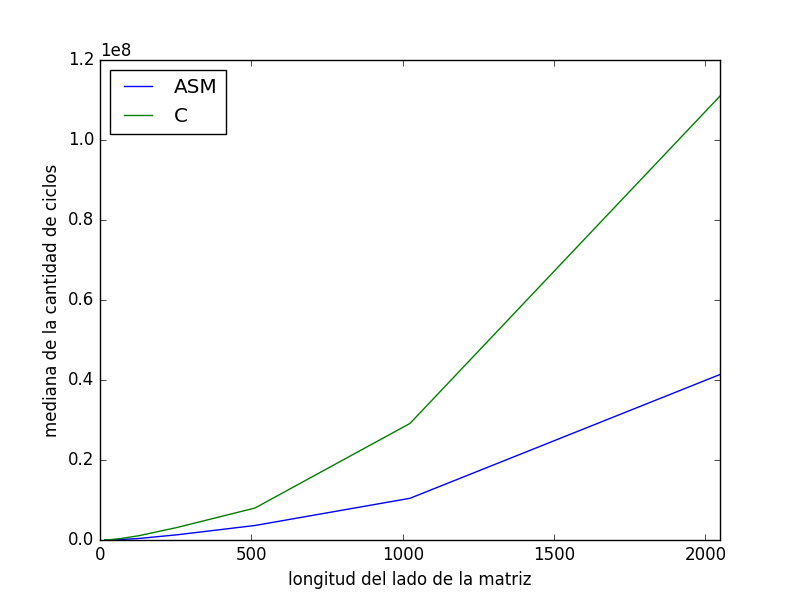
\includegraphics[width=12.5cm, height=9
cm]{images/car_tresColores.png}
\end{center}
\vspace{6px}


Como podemos observar la diferencia entre ASM y C es notoria. Esto se debe al paralelismo que se maneja en las instrucciones de SSE que se propuso utilizar en este trabajo. 

\subsection{Efecto Bayer}

La segunda experimentación que se realizó fue con el filtro de $Efecto$ $Bayer$, este mismo filtro deja solo uno de los 3 colores representantes de los píxeles con un patrón determinado. Como primera idea de las posibles mejoras que surgen a partir de utilizar ASM en vez de C, son los accesos a memoria. En general la cantidad de accesos a memoria se reduce, ya que trabajamos con múltiples píxeles al mismo tiempo. Este filtro no es la excepción y al traer de memoria 4 píxeles en vez de 1, como se haría con C, se mejoran mucho los tiempos. Continuemos con los resultados:


\vspace{6px}
\begin{center}
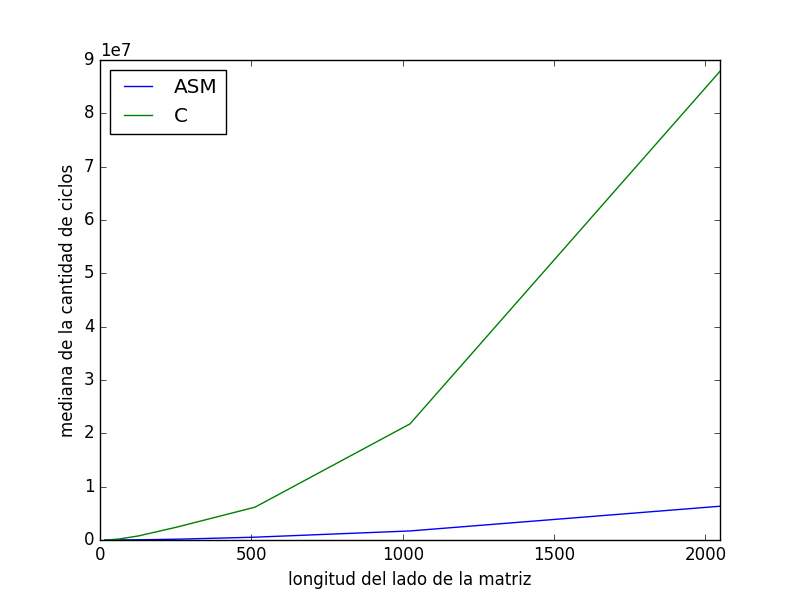
\includegraphics[width=12.5cm, height=9
cm]{images/car_efectoBayer.png}
\end{center}
\vspace{6px}

Podemos observar como el cambio es bastante alto con respecto a la implementación en C. Esto se debe, principalmente, a los accesos a memoria. Sin embargo, las operaciones que realizan las instrucciones de SSE influyen en los cambios de tiempo ya que se realizan simultáneamente.



\subsection{Edge Sobel}

La cantidad de operaciones que se realizan sobre en este filtro es bastante más que las que venimos trabajando anteriormente, por lo que uno de los posibles cambios en comparación con C, es que en ASM va a mejorar bastante el tiempo.


\vspace{6px}
\begin{center}
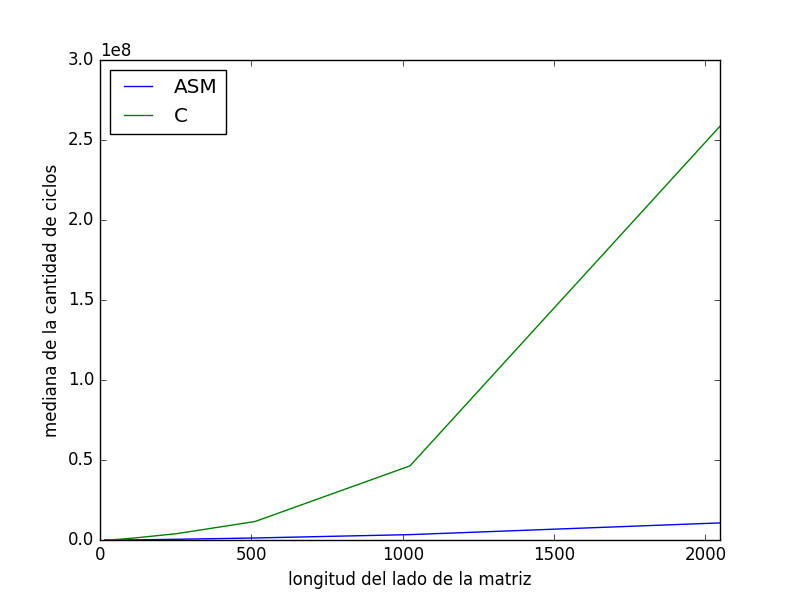
\includegraphics[width=12.5cm, height=9
cm]{images/car_edgeSobel.png}
\end{center}
\vspace{6px}





\subsection{Cambia Color}

En el caso de $Cambia$ $Color$ esperamos un cambio considerable ya que los accesos a memoria que se realizan dentro de cada iteración son 2, uno para traer los datos y otro para escribir. 

\vspace{6px}
\begin{center}
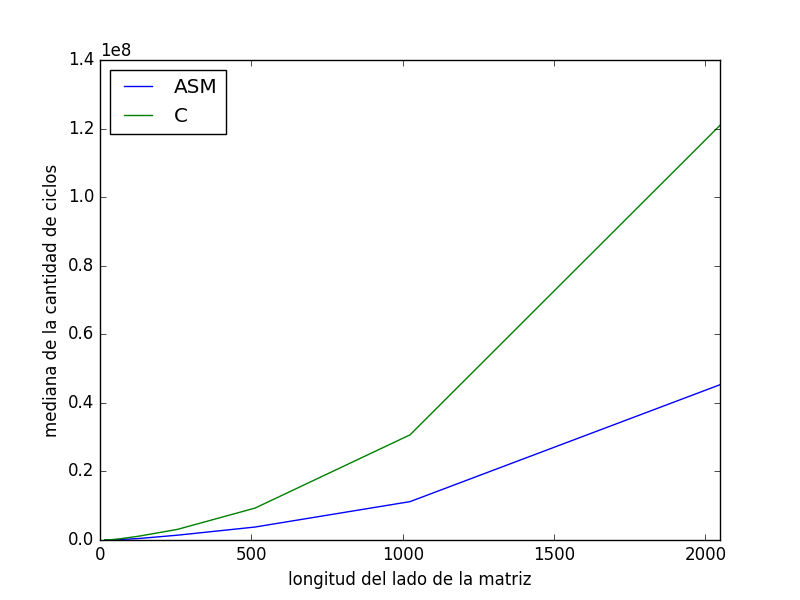
\includegraphics[width=12.5cm, height=9
cm]{images/car_cambiaColor.png}
\end{center}
\vspace{6px}

Podemos ver que el cambio es considerable, aunque no tanto como en otros filtros. Luego de un análisis se llegó a la conclusión de que el cambio de tiempos es bueno, aunque no mejor que otros filtros, debido a la cantidad de operaciones que tiene una iteración a comparación de los demás filtros. 
%\newpage

%Backtracking
\section{Conclusiones}
Como conclusión general, podemos ver como los cambios en ASM y C se pronuncian en cada uno de los filtros. Así vemos como poder trabajar a más bajo nivel para situaciones específicas puede resultar muy beneficioso si lo que buscamos es optimizar los tiempos, como contraparte es más complejo trabajar en ASM que en C.


\subsection{Tres Colores y Cambia Color}

En estos dos filtros encontramos similitudes con respecto a los tiempos de corrida. 
Se puede observar en el siguiente gráfico como sus tiempos se asemejan bastante entre sí, a pesar de ser diferentes filtros. 

\vspace{6px}
\begin{center}
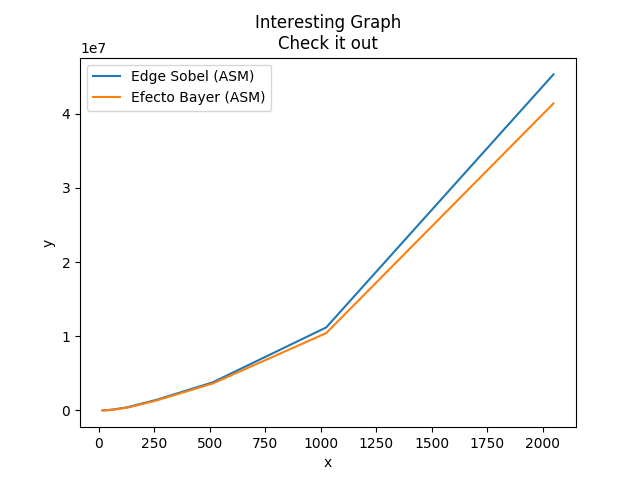
\includegraphics[width=12.5cm, height=9
cm]{images/cambia_tres.png}
\end{center}
\vspace{6px}


Uno de los primeros enfoques que surgieron a partir de esta comparación es revisar el código de cada uno de los filtros y pensar que tan complejas son las intrucciones que realiza. 
Ambos filtros tienen instrucciones como $shuffle$ que tienen un costo mucho mayor a instrucciones mas sencillas como $pand$ o $padd$. Cabe destacar también, que ambos filtros realizan pocos accesos a memoria. Esto es clave a la hora de hablar de tiempos de ejecución, ya que el tiempo que se tarda en ir a la memoria es mucho mayor a solamente trabajar dentro de registros del procesador por la proximidad de los mismos. 



\subsection{Edge Sobel y Efecto Bayer}

Sobre estos filtros también encontramos similitudes en tiempos de ejecución. Ambos filtros realizan instrucciones en general sencillas, con pocos $shuffle$ y sin conversiones de datos. Podemos ver en el siguiente gráfico las similitudes:


\vspace{6px}
\begin{center}
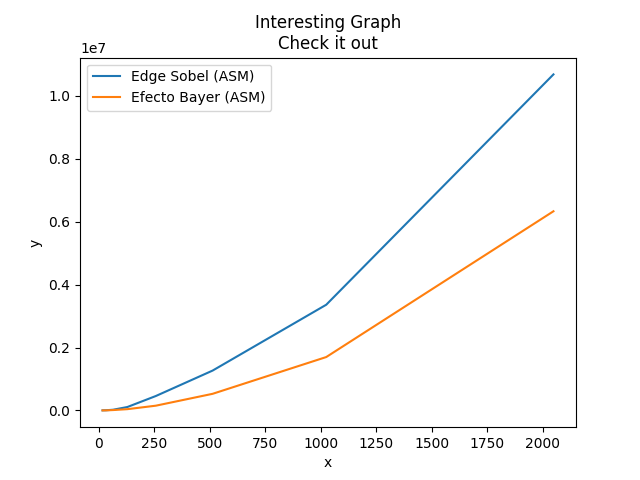
\includegraphics[width=12.5cm, height=9
cm]{images/sobel_bayer.png}
\end{center}
\vspace{6px}


A partir de estos resultados y sabiendo que las instrucciones que se realizan en ambos filtros son de "costos similares", a pesar de no tener la misma cantidad de instrucciones, podemos ver como los tiempos se asemejan lo suficiente como para pensar que es por la similitud en complejidad de dichas instrucciones. Esto significa que ambas tienen tiempos similares debido a que ambas utilizan instrucciones poco costosas de ASM. 


\subsection{Sobre los 4 filtros}

Como una conclusón general nos gustaría hacer una comparación entre $Cambia$ $Color$ y $Tres$ $Colores$ contra $Edge$ $Sobel$ y $Efecto$ $Bayer$. 
Entre ambos grupos podemos notar una diferencia grande en los tiempos de ejecución en ASM. 
Nuestro principal hipótesis sobre dicha diferencia en las complejidad de las intrucciones que tienen a cargo cada uno de los grupos de filtros. En el primero grupo ($Cambia$ $Color$ y $Tres$ $Colores$) tenemos instrucciones como $shuffle$ que a diferencia del segundo grupo ($Edge$ $Sobel$ y $Efecto$ $Bayer$) no se encuentran tan seguido en cada iteración como en el primer grupo. Otro punto a destacar sobre el mismo eje son las conversiones de datos, en el segundo grupo no se realiza ninguna conversión de datos a diferencia del primero, donde de momento se trabaja en $int$ y en otros necesitamos la precisión de los $floats$. 
%\newpage

\end{document}
